\documentclass{article}
\usepackage{graphicx}
\usepackage[margin=1.5cm]{geometry}
\usepackage{amsmath}

\begin{document}
\twocolumn

\title{Wednesday warm-up: displacement, velocity, and acceleration vectors}
\author{Prof. Jordan C. Hanson}

\maketitle

\section{Memory Bank}

\begin{enumerate}
\item $\Delta x = \vec{x}_f - \vec{x}_i$ ... Definition of displacement
\item $\Delta t = t_f - t_i$ ... Definition of time duration
\item $\vec{v} = \Delta \vec{x} / \Delta t$ ... Definition of vector velocity
\item $\vec{a} = \Delta \vec{v} / \Delta t$ ... Definition of vector acceleration
\end{enumerate}

\section{Velocity as a vector}

\begin{enumerate}
\item Suppose the location of an aircraft is described by a 2D coordinate system in which East corresponds to the postive x-axis, and North corresponds to the positive y-axis.  An aircraft takes off from the origin in a direction 60 degrees above the x-axis (60 degrees North of East), with a speed of 200 km/hr.
\begin{enumerate}
\item Determine the components of the velocity vector, $v_x$ and $v_y$, and build the velocity vector $\vec{v} = v_x \hat{i} + v_y \hat{j}$. \\ \vspace{1.5cm}
\item What is the location of the aircraft after 12 minutes? \\ \vspace{1.5cm}
\item The pilot turns the aircraft due East, and travels at the same \textit{speed} of 200 km/hr for another 6 minutes.  What is the final location? \\ \vspace{1.5cm}
\end{enumerate}
\end{enumerate}

\section{Acceleration}

\begin{enumerate}
\item A vehicle with different velocity and \textit{acceleration} vectors is shown in Fig. \ref{fig:vehicle_v_a}.  Match the pictures to the following statements.  (1) The vehicle is moving to the right and speeding up.  (2) The vehicle is moving to the right and slowing down.  (3) The vehicle is moving to the left and speeding up. (4) The vehicle is moving to the left and slowing down.
\begin{figure}[hb]
\centering
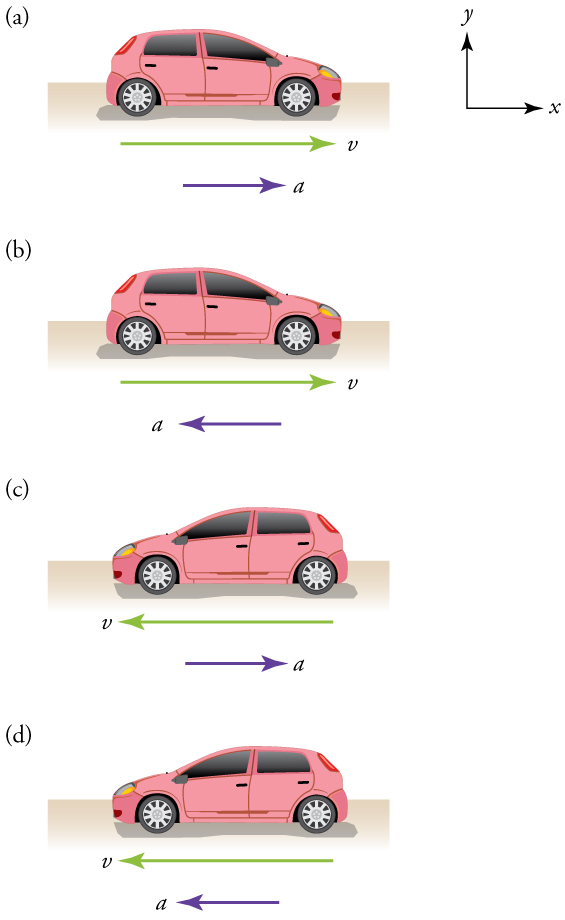
\includegraphics[width=0.33\textwidth,trim=0cm 0cm 1.75cm 0cm,clip=true]{figures/vehicle_v_a.jpeg}
\caption{\label{fig:vehicle_v_a} Four cases of velocity and acceleration in one dimension.}
\end{figure}
\item Suppose the velocity of the vehicle in Fig. \ref{fig:vehicle_v_a} is 40 km hr$^{-1}$ at $t=0$ seconds, and 80 km hr$^{-1}$ at $t=5$ seconds. (a) What is the acceleration in km hr$^{-1}$ s$^{-1}$? (b) What is the acceleration in m s$^{-2}$?
\end{enumerate}

\end{document}
